\documentclass[crop,tikz]{standalone}

\tikzset{>=latex}
\usetikzlibrary{decorations.markings}
\colorlet{green}{black!40!green}

\begin{document}
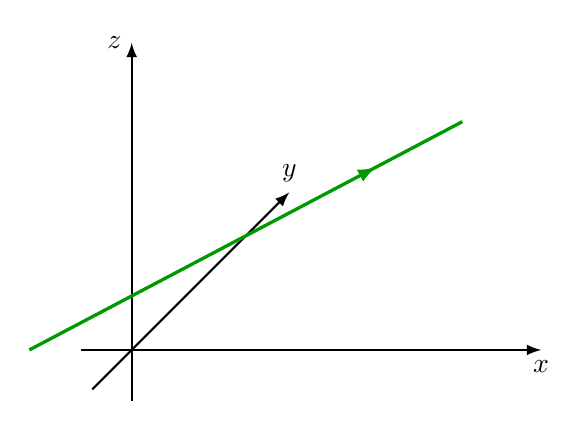
\begin{tikzpicture}[scale=1.3]
  % axes
  \draw[->,thick] (xyz cs:x=-0.5) -- (xyz cs:x=4)  node[below] {$x$};
  \draw[->,thick] (xyz cs:y=-0.5) -- (xyz cs:y=3)  node[left]  {$z$};
  \draw[->,thick] (xyz cs:z=1)    -- (xyz cs:z=-4) node[above] {$y$};
  % path
  \draw[red,very thick,
        decoration={markings, mark=at position 0.8 with {\arrow{>}}},
        postaction={decorate},
        green]
       (xyz cs:x=-1) -- (xyz cs:x=4,y=3,z=2);
\end{tikzpicture}
\end{document}
